\documentclass[aspectratio=169]{beamer}

\mode<presentation>

\usepackage[utf8]{inputenc}
\usepackage[T1]{fontenc}	%makes å,ä,ö etc. proper symbols
\usepackage{amsmath}
\usepackage{graphicx}
\usepackage{xcolor}
\usepackage{listings}
\usepackage{multicol}
\usepackage{hyperref}
\usepackage[swedish]{babel}

\definecolor{LundaGroen}{RGB}{00,68,71}
\definecolor{StabilaLila}{RGB}{85,19,78}
\definecolor{VarmOrange}{RGB}{237,104,63}

\definecolor{MagnoliaRosa}{RGB}{251,214,209}
\definecolor{LundaHimmel}{RGB}{204,225,225}
\definecolor{LundaLjus}{RGB}{255,242,191}

\usefonttheme{serif}
\usetheme{malmoe}
\setbeamercolor{palette primary}{bg=LundaHimmel, fg=StabilaLila}
\setbeamercolor{palette quaternary}{bg=LundaGroen, fg=MagnoliaRosa}
\setbeamercolor{background canvas}{bg=LundaLjus}
\setbeamercolor{structure}{fg=LundaGroen}

\usepackage[many]{tcolorbox}

\newtcolorbox{cross}{blank,breakable,parbox=false,
  overlay={\draw[red,line width=5pt] (interior.south west)--(interior.north east);
    \draw[red,line width=5pt] (interior.north west)--(interior.south east);}}
    
\newcommand{\code}[1]{\colorbox{white}{\lstinline{#1}}}



\lstset{language=Python} 
\lstset{%language=[LaTeX]Tex,%C++,
    morekeywords={PassOptionsToPackage,selectlanguage,True,False},
    keywordstyle=\color{blue},%\bfseries,
    basicstyle=\small\ttfamily,
    %identifierstyle=\color{NavyBlue},
    commentstyle=\color{red}\ttfamily,
    stringstyle=\color{VarmOrange},
    numbers=left,%
    numberstyle=\scriptsize,%\tiny
    stepnumber=1,
    numbersep=8pt,
    showstringspaces=false,
    breaklines=true,
    %frameround=ftff,
    frame=single,
    belowcaptionskip=.75\baselineskip,
	tabsize=4,
	backgroundcolor=\color{white}
    %frame=L
}
\lstset{
	escapeinside={(*@}{@*)}
}
\begin{document}

\lstset{literate=
  {á}{{\'a}}1 {é}{{\'e}}1 {í}{{\'i}}1 {ó}{{\'o}}1 {ú}{{\'u}}1
  {Á}{{\'A}}1 {É}{{\'E}}1 {Í}{{\'I}}1 {Ó}{{\'O}}1 {Ú}{{\'U}}1
  {à}{{\`a}}1 {è}{{\`e}}1 {ì}{{\`i}}1 {ò}{{\`o}}1 {ù}{{\`u}}1
  {À}{{\`A}}1 {È}{{\'E}}1 {Ì}{{\`I}}1 {Ò}{{\`O}}1 {Ù}{{\`U}}1
  {ä}{{\"a}}1 {ë}{{\"e}}1 {ï}{{\"i}}1 {ö}{{\"o}}1 {ü}{{\"u}}1
  {Ä}{{\"A}}1 {Ë}{{\"E}}1 {Ï}{{\"I}}1 {Ö}{{\"O}}1 {Ü}{{\"U}}1
  {â}{{\^a}}1 {ê}{{\^e}}1 {î}{{\^i}}1 {ô}{{\^o}}1 {û}{{\^u}}1
  {Â}{{\^A}}1 {Ê}{{\^E}}1 {Î}{{\^I}}1 {Ô}{{\^O}}1 {Û}{{\^U}}1
  {œ}{{\oe}}1 {Œ}{{\OE}}1 {æ}{{\ae}}1 {Æ}{{\AE}}1 {ß}{{\ss}}1
  {ű}{{\H{u}}}1 {Ű}{{\H{U}}}1 {ő}{{\H{o}}}1 {Ő}{{\H{O}}}1
  {ç}{{\c c}}1 {Ç}{{\c C}}1 {ø}{{\o}}1 {å}{{\r a}}1 {Å}{{\r A}}1
  {€}{{\euro}}1 {£}{{\pounds}}1 {«}{{\guillemotleft}}1
  {»}{{\guillemotright}}1 {ñ}{{\~n}}1 {Ñ}{{\~N}}1 {¿}{{?`}}1
}

% NEW COMMANDS
\newcommand{\fortt}{\texttt{for}}
\newcommand{\whilett}{\texttt{while}}
\newcommand{\iftt}{\texttt{if}}

\AtBeginSection[ ]
{
\begin{frame}{Outline}
    \tableofcontents[currentsection]
\end{frame}
}

\title{Köer}
\date{vt 24}
\author{Programmering 2}

\maketitle

\tableofcontents

\section{Köer}

\subsection{Vad är en kö?}

\begin{frame}
	\frametitle{Kö}
	
	En \textit{kö} är en datastruktur där varje element refererar till ett annat element, som en i stack. Skillnaden mellan en kö och en stack är att i en kö så är det ''först in först ut'' (FIFO) som gäller.
	
\end{frame}

\begin{frame}
	\frametitle{Exempel}
	
	En vanlig \textit{kö} IRL är kön till kassan i en affär. Där ställer man sig på led och den som kom först blir betjänad först.
	
\end{frame}

\subsection{Metoder}

\begin{frame}
	\frametitle{Kö}
	
	En \textit{kö} har följande fyra metoder:
	
	\begin{enumerate}
		\item put (enqueue)
		\item get (dequeue)
		\item front
		\item rear
	\end{enumerate}
	
\end{frame}


\begin{frame}
	\frametitle{Metoder}
	
	\begin{itemize}[<+->]
		\item Metoden \texttt{put} lägger till ett element sist i \textit{kön}. Du kan jämföra det med metoden \texttt{append} i listor.
		
		\item Metoden \texttt{get} plockar bort det första elementet i \textit{kön}. Du kan jämföra det med motsvarande metod i listor.
		
		\item Metoden \texttt{front} tittar på det första elementet i \textit{kön} och ger värdet.
	
		\item Metoden \texttt{rear} tittar på det sista elementet i \textit{kön} och ger värdet.
		
		En kö måste inte ha metoden \texttt{rear}
	\end{itemize}
	
\end{frame}


\section{Köer och listor}

\subsection{Listor som köer}

\begin{frame}[fragile]
	\frametitle{Listor som köer}
	\framesubtitle{Listor}

	I Python kan du simulera en \textit{kö} med en lista. Det är ganska enkelt eftersom listan har alla metoder en \textit{kö} har och lite till.
	
	\begin{lstlisting}
kö = []
kö.append(4) # Motsvarar put
kö.pop(0) # Motsvarar get
kö[0] # Motsvarar front
kö[-1] # Motsvarar rear
	\end{lstlisting}
	
\end{frame}
	
\subsection{Nackdelen med listor}
	
\begin{frame}
	\frametitle{Köer och listor}
	\framesubtitle{Nackdelen med listor}
	
	Nackdelen med listor är att listor är en sammanhängande grupp i minnet på datorn. Så om man lägger till något i en lista så tar det mer plats i minnet -- vilket är som det ska -- men om det nu skulle krocka med en annan sak lagrat i minnet så allokerar man en ny plats i minnet och flyttar hela listan i minnet. Detta gör att operationer på listor kan ta väldigt olika lång tid, om datorn måste flytta på hela listan i minnet.

\end{frame}

\subsection{Fördelen med köer}

\begin{frame}
	\frametitle{Köer och listor}
	\framesubtitle{Fördelen med köer}
	
	\textit{Köer} däremot lagrar varje element separat i minnet, det kan ge lite mer overhead i varje element. Men det gör att man riskerar inte att flytta på hela \textit{kön} när man lägger till element i den. Detta gör att operationer med \textit{köer} är konsekventa i hur lång tid de tar att genomföra.
	
\end{frame}

\subsection{Kö vs. Stack}

\begin{frame}
	\frametitle{Kö vs. stack}

	\centering
	
	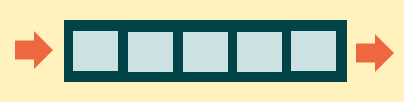
\includegraphics[width=.45\textwidth]{queue-illustration.png}
	
	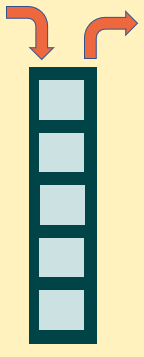
\includegraphics[width=.15\textwidth]{stack-illustration.png}
	
\end{frame}

\section{Övningar}

\subsection{Instruktioner och klassdiagram}

\begin{frame}[fragile]
	\frametitle{Övningar}
	
	Skapa din egna \texttt{queue}-klass. Du får en driver kod på Vklass döpt till \texttt{kö.py}
	
	Här ser du klassdiagramen för klasserna \texttt{Node} och \texttt{Queue}
	
	\begin{center}
		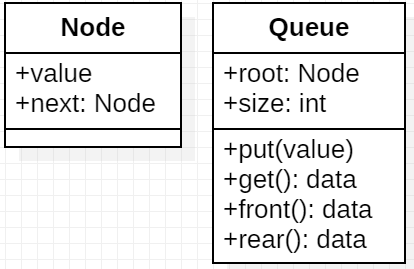
\includegraphics[width=.4\textwidth]{kö.png}
	\end{center}
	
	En del implementationer har istället för attributet \texttt{root} attributen \texttt{first} och \texttt{last}. Genom att använda \texttt{last} kan man korta ner tiden det tar att lägga till ett nytt element.
	
\end{frame}



\end{document}